\chapter{Dynamique}
\label{sec:dynamic}

Chapitre en construction!


\section{Equations of motion in joint-space}
%\section{Équations du mouvement dans l'espace des joints}
\label{sec:eom}

The general form of the equations of motion of robotic systems (interconnected rigid body driven by motors) is:
%
\begin{align}
H(\col{q}) \col{\ddot{q}} + C(\col{q},\col{\dot{q}}) \col{\dot{q}} + D \col{\dot{q}} + \col{g}(\col{q}) = B(\col{q}) \col{\tau} 
\label{eq:manipulator}
\end{align}
%
where $\col{q}$ is the generalized coordinates vector, $H$ is the inertia matrix, $C$ is the Coriolis/centrifugal force matrix, $D$ is a damping matrix, $\col{g}$ is the gravitational forces vector and $B$ is a matrix mapping motor torques $\col{\tau}$ into generalized forces.
%
Kinetic energy is given by:
%
\begin{align}
\frac{1}{2} \col{\dot{q}}^T H(\col{q}) \col{\dot{q}} 
\label{eq:kinetic}
\end{align}
%
Conservation of energy also give the following relation:
%
\begin{align}
\dot{H} = C + C^T
\label{eq:cener}
\end{align}
%
On occasion, dependence notation is dropped and $\col{c}$ is used to represent all state dependent forces, leading to the short form:
%
\begin{align}
H \col{\ddot{q}} + \col{c} = B \col{\tau} 
\label{eq:manipulator_short}
\end{align}

\subsection{Coordinate systems}
\label{sec:coord}

%Fig. \ref{fig:coord} shows all the used coordinates systems. 
%
\begin{figure}[t]
	\centering
		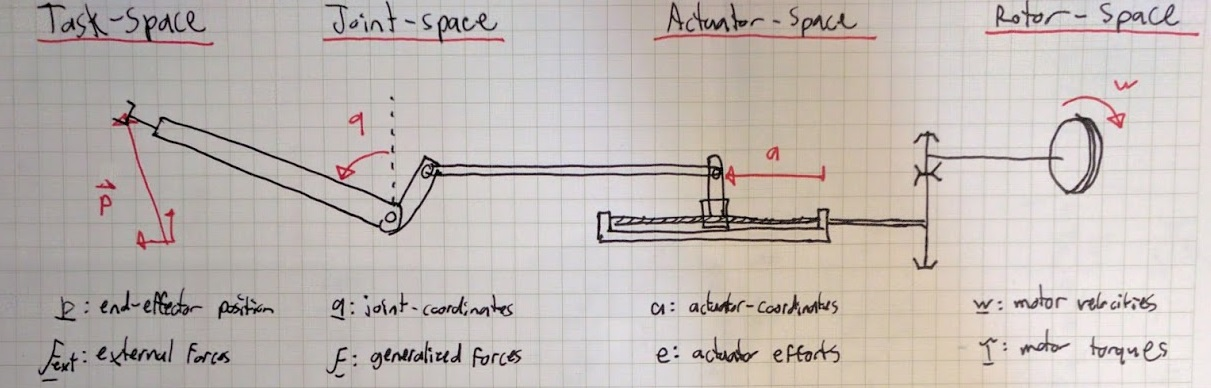
\includegraphics[width=0.99\textwidth]{coord.jpg}
	\caption{Coordinate systems}%
	\label{fig:coord}
\end{figure}
%
The following equation represents the most general case:
%
\begin{align}
H \col{\ddot{q}} + C \col{\dot{q}} + D \col{\dot{q}} + \col{g} =  \underbrace{ J_a^T(\col{q}) R^T }_{B(\col{q})}  \col{\tau} + J_e^T(\col{q}) \col{f}_e + J_c^T(\col{q}) \col{f}_c
\label{eq:manipulator_gen}
\end{align}
%
Where coordinates transforms are defined by:
%
\begin{align}
\col{\dot{r}}   &= J_e( \col{q} ) \col{\dot{q} }  \quad \text{ from joint-space to end-effector   } \\
\col{\dot{a}}   &= J_a( \col{q} ) \col{\dot{q} }  \quad \text{ from joint-space to actuator-space } \\
\col{w }        &= R              \col{\dot{a} }  \quad\quad \text{ from actuator-space to rotor-space } 
\label{eq:coord_transform2}
\end{align}
%

\newpage
\subsection{Contact}
\label{sec:contact}

This section presents equations for representing contact situations.

\subsubsection{Kinematic constraints}
\label{sec:constraints}
%
If a robotic manipulator enter contact with a fixed object, then some DoF are constrained. In the case of a bilateral constraint, the constraint can be expressed as:
\begin{align}
\col{\phi}( \col{ q } ) = 0
\label{eq:constraint}
\end{align}
%
The time-derivative of the constraint must also be equal to zero, which gives some constraints in terms of velocity and acceleration:
\begin{align}
\frac{d \col{\phi}( \col{ q } ) }{dt}     &= J_c( \col{ q } ) \col{\dot{q}}  = 0 \\
\frac{d^2 \col{\phi}( \col{ q } ) }{dt^2} &= J_c( \col{ q } ) \col{\ddot{q}}  + \dot{J}_c( \col{ q } ) \col{\dot{q}} = 0 
\label{eq:constraint_diff}
\end{align}
%
when $J_c$ is the constraint Jacobian:
%
\begin{align}
J_c( \col{ q } )                    &= \frac{d \col{\phi}( \col{ q } ) }{d\col{ q }}
\label{eq:constraint_jaco}
\end{align}

\subsubsection{Constraint forces}
\label{sec:constraint_forces}

The constraint Jacobian can be used to map constraint forces $\col{f}_c$ to generalized forces in the EoM:
%
\begin{align}
H \col{\ddot{q}} + \col{c} = B \col{\tau} + J_c( \col{ q } )^T  \col{f}_c
\label{eq:manipulator_constraint}
\end{align}
%
Solving for $\col{\ddot{q}}$ in eq. \eqref{eq:manipulator_constraint} and substituting in eq. \eqref{eq:constraint_diff}, it is possible to get and expression for the constraint forces $\col{f}_c$ as a function of states and applied torques:
%
\begin{align}
\col{f}_c = \left( J_c H^{-1} J_c^T \right)^{-1} \left(  J_c H^{-1} [\col{c} - B \col{\tau} ] - \dot{J}_c( \col{ q } ) \col{\dot{q}}   \right)
\label{eq:const_forces}
\end{align}
%
Alternatively, it possible to solve for acceleration $\col{\ddot{q}}$ and constraints forces $\col{f}_c$ simultaneously by solving the following system of equations:
%
\begin{align}
\left[ \begin{array}{c c } 	H & -J_c^T  \\ J_c 	& 0  	\end{array} \right] \left[ \begin{array}{c} \col{\ddot{q}}  \\ \col{f}_c \end{array} \right] = \left[ \begin{array}{c}  B \col{\tau} - \col{c}   \\ -\dot{J}_c \col{\dot{q}}  \end{array} \right]
\label{eq:manipulator_constraint_eom}
\end{align}


\subsubsection{Impact impulsive behavior}
\label{sec:impact}
%
When the robot first enters contact with a fixed object, impulsive contact forces will act on the system. Integrating eq. \eqref{eq:manipulator_constraint} over the short impact interval gives:
%
\begin{align}
\int{ ( H \col{\ddot{q}} + \col{c} ) dt } &= \int{ ( B \col{\tau} + J_c( \col{ q } )^T  \col{f}_c ) dt } \\
H \col{\dot{q}}^+ - H \col{\dot{q}}^- &= J_c( \col{ q } )^T  \int{  \col{f}_c dt }
\label{eq:manipulator_impact}
\end{align}
%
where any non-impulsive forces are neglected during the short impact interval. Projecting onto constrained coordinates (multiplying by $J_c H^{-1}$) gives:
%
\begin{align}
J_c \col{\dot{q}}^+ - J_c \col{\dot{q}}^- &= J_c H^{-1} J_c^T  \int{  \col{f}_c dt }
\label{eq:manipulator_impact2}
\end{align}
%
Then assuming a sticky inelastic impact (no bouncing), then the constraint is respected after the impact ($J_c \col{\dot{q}}^+=0$) and it is possible to solve for the impact force:
%
\begin{align}
\int{  \col{f}_c dt } &= - \left( J_c H^{-1} J_c^T \right)^{-1}  J_c \col{\dot{q}}^-
\label{eq:manipulator_impact_force}
\end{align}
%
and also for the velocity after the impact:
%
\begin{align}
\col{\dot{q}}^+ &= - \Big[ I - H^{-1} J_c^T \left( J_c H^{-1} J_c^T \right)^{-1} J_c \Big] \col{\dot{q}}^-
\label{eq:manipulator_impact_velocity}
\end{align}
%
Or change in velocity:
%
\begin{align}
\Delta \col{\dot{q}} &=  \Big[ H^{-1} J_c^T \left( J_c H^{-1} J_c^T \right)^{-1} J_c \Big] \col{\dot{q}}^-
\label{eq:manipulator_impact_velocity_delta}
\end{align}
%

Alternatively, it possible to solve for velocity $\col{\dot{q}}^+$ and impulsive forces $\int{ \col{f}_c dt }$ simultaneously by solving the following system of $n+c$ equations:
%
\begin{align}
\left[ \begin{array}{c c } 	H & -J_c^T  \\ J_c 	& 0  	\end{array} \right] \left[ \begin{array}{c} \col{\dot{q}}^+  \\ \int{ \col{f}_c dt }\end{array} \right] = \left[ \begin{array}{c}  	H \col{\dot{q}}^-   \\ 0  \end{array} \right]
\label{eq:manipulator_impact_eom}
\end{align}

\begin{table}[htbp]
	\centering
	\caption{Nomenclature pour la dynamique dans l'espace des joints}	% Table caption must be placed on top of the table %
		\begin{tabular}{ c c l r }
        \hline \hline
				\multicolumn{4}{c}{Scalars} \\
				\hline \hline
			$n$             &  :  & number of DoF                                              & \\
			$m$             &  :  & number of actuators                                        & \\
			$c$             &  :  & number of contact constraints                              & \\
			$o$             &  :  & number of end-effector coordinates                         & \\ 
			$i$             &  :  & index for DoF                                              & \\ 
			\hline \hline
			\multicolumn{4}{c}{Vectors} \\
			\hline \hline
			$\col{\tau}$    &  :  & Actuator forces/torques                                    & $m$  \\
			$\col{q}$       &  :  & Joint coordinates position vector                          & $n$  \\
			$\col{w}$       &  :  & Actuator coordinates velocity vector                          & $m$  \\ 
			$\col{g}$       &  :  & Gravitational forces vector                                & $n$  \\
			$\col{c}$       &  :  & Sum of state-dependent generalized forces                  & $n$  \\
			$\col{\phi}$    &  :  & Constraint vector                                          & $c$  \\
			$\col{f}_c$     &  :  & Contact forces vector                                      & $c$  \\
			$\col{f}_e$     &  :  & End-effector external forces vector                        & $o$  \\
			$\col{r}$       &  :  & End-effector position vector                               & $o$  \\
			\hline \hline
			\multicolumn{4}{c}{Matrices} \\
			\hline \hline
			$H$             &  :  & Inertia matrix                                             & $n$ x $n$ \\
			$D$             &  :  & Damping matrix                                             & $n$ x $n$ \\
			$C$             &  :  & Coriolis/Centrifugal forces matrix                         & $n$ x $n$ \\
			$B$             &  :  & Generalized forces matrix                                  & $n$ x $m$ \\
			$J_a$           &  :  & Actuator coordinates / joint coordinates Jacobian matrix   & $m$ x $n$ \\
			$J_e$           &  :  & Task-space coordinates / joint coordinates Jacobian matrix & $o$ x $n$ \\
			$J_c$           &  :  & Contact constraints Jacobian matrix                        & $c$ x $n$  \\
		\hline \hline
        \end{tabular}		
	\label{tab:nom}
\end{table}




\newpage
\section{Hybrid system dynamics}

Hybrid dynamical system can be represented in the general form:
%
\begin{align}
\text{Continuous evolution: } \left(  \dot{\col{x}} , \dot{k} \right) &=  \left( \, f_k( \col{x} , \col{u} , \col{d} ) \, , \, 0 \, \right) \\
\text{Discrete jumps: } \left(  \col{x}^+ , k^+ \right) &=  \left( h_{ij}( \col{x}^- , \col{u}^- ) , j \right) \quad\text{if}\quad \left(  \col{x} , k , \col{u} \right) \in D_{ij}  
\end{align}
%
where $\col{x}$ is a continuous state vector, and $k$ is a discrete mode and $D_{ij}$ is the domain mapping conditions leading to a transition $k:i \rightarrow j$. For robotic systems, the discrete mode can represent discrete configurations of the robot , like discrete modes in the control law or contact/non-contact conditions. The jump map then represents the impulsive response when contact is made. 

\subsection{Switched system}

A restricted class of hybrid system, called switched system, are hybrid systems for which the jump map for continuous state is the identify function:
%
\begin{align}
\text{Continuous evolution: } \left(  \dot{\col{x}} , \dot{k} \right) &=  \left( \, f_k( \col{x} , \col{u} , \col{d} ) \, , \, 0 \, \right) \\
\text{Discrete jumps: } \left(  \col{x}^+ , k^+ \right) &=  \left( \col{x}^- , j \right) \quad\text{if}\quad \left(  \col{x} , k , \col{u} \right) \in D_{ij} 
\end{align}
%

\subsubsection{Switched system where the discrete mode is a control input}

In the situation where the discrete operating mode $k$ is a control input, then there is no need to keep track of discrete mode evolution and only the piece-wise continuous differential equations are sufficient to model the system evolution:
%
\begin{align}
\dot{\col{x}} = f_k( \col{x} , \col{u} , \col{d} ) 
\end{align}
%
A robot with a continuous dynamics but with a control law using discrete modes of operation would be of this category. 
